\documentclass{article}
\usepackage{amsmath}
\usepackage{graphics}
\graphicspath{{./}}
\DeclareGraphicsExtensions{.pdf, .png, .jpg}
\usepackage{mathtext}
\usepackage[english,russian]{babel}
\usepackage[T2A]{fontenc}
\usepackage[utf8]{inputenc}
\setcounter{MaxMatrixCols}{20}
\begin{document}
	$A$ -- прямоугольная матринца размером $m \times n$
	$$
	A =
	\begin{pmatrix}
		1 0 0 0 1 0 0 0 0 0 0 0 0 0 0\\
		0 1 0 0 0 1 0 0 0 0 0 1 0 0 0\\
		0 0 0 0 0 0 1 1 0 0 1 0 0 0 0\\
		0 0 0 0 0 0 0 0 1 0 0 0 1 1 0\\
		0 0 1 0 0 0 0 0 0 1 0 0 0 0 0\\
		0 0 0 1 0 0 0 0 0 0 0 0 0 0 1
	\end{pmatrix}
	$$
	Матрица $B$ --- прямоугольная матрица размеро $m \times n$ где $m$ -- число элементов $n$ -- число выводов
	$$
	B =
	\begin{pmatrix}
		1 1 1 1 0 0 0 0 0 0 0 0 0 0 0\\
		0 0 0 0 1 1 1 0 0 0 0 0 0 0 0\\
		0 0 0 0 0 0 0 1 1 1 0 0 0 0 0\\
		0 0 0 0 0 0 0 0 0 0 1 1 1 0 0\\
		0 0 0 0 0 0 0 0 0 0 0 0 0 1 1
	\end{pmatrix}
	$$
	Представление коммутационной схемы в виде Графа элементных комплексов

	Матрица $Q$ --- прямоугольная матрица размером $m_1 \times m$

	$$
	Q =
	\begin{pmatrix}
		1 & 1 & 0 & 0 & 1 & 1\\
		1 & 1 & 1 & 0 & 0 & 0\\
		0 & 0 & 1 & 1 & 1 & 0\\
		0 & 1 & 1 & 1 & 0 & 0\\
		0 & 0 & 0 & 1 & 0 & 1
	\end{pmatrix}
	$$
	$$
	Q = B A^T
	$$

	Взвешенный граф схемы

	% Тут должен быть граф
	%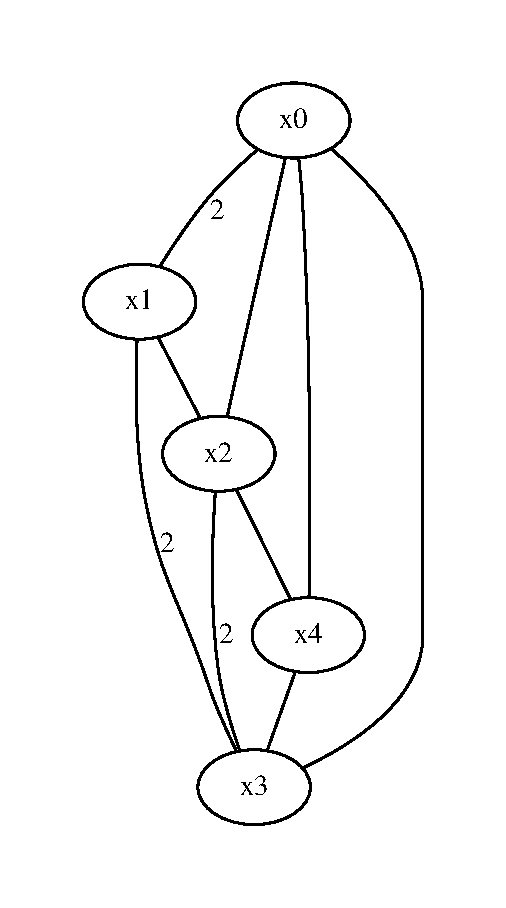
\includegraphics{lection5.1.pdf}
	
	$R$ -- матрица взвешенного графа
	$$
	R = \begin{pmatrix}
		0 & 2 & 1 & 1 & 1\\
		2 & 0 & 1 & 2 & 0\\
		1 & 1 & 0 & 2 & 1\\
		1 & 2 & 2 & 0 & 1\\
		1 & 0 & 1 & 1 & 0
	\end{pmatrix}
	$$

	$$
	\widetilde{R} = Q Q^T
	$$
	
	Матрица $\widetilde{R}$ всегда отличается от матрицы $R$ только элементами главной диагонали

	$$
	x_0 \to \left\{x_1, x_2, x_3, x_4\right\}
	$$
	$$
	x_1 \to \left\{ x_0, x_2< x_3\right\}
	$$
	$$
	x_2 \to \left\{x_0, x_1, x_2, x_4\right\}
	$$
	$$
	x_3 \to \left\{x_0, x_1, x_2, x_4\right\}
	$$
	$$
	x_4 \to \left\{x_0, x_2, x_3\right\}
	$$
	$Z$ -- массив отображений
	%$$
	%Z = \left[
	%\begin{array}
	%1&2&3&4&0&2&3&0&1&3&4&0&1&2&4&0&2&3
	%\end{array}
	%\right]
	%$$
	$W$ -- массив весовых коэфициентов
	%$$
	%W = \left[2 1 1 1 2 1 2 1 1 2 1 1 2 2 1 1 1 1\right]
	%$$
	$V$ -- массив границ
	%$$
	%v = \left[4 7 11 15 18\right]
	%$$
	
	Реализация на Matlab алгоритмов преобразования различных видов информации

	%S = \[1,0, 1; 1, 1, 1; 2, 1, 2; 2, 3, 2; 3, 1, 3; 3, 2, 1; 3, 3, 1; 4, 2, 2; 4, 3, 3; 4, 4, 1; 5, 0, 3; 5, 2, 3; 6, 0, 4; 6, 4, 2\]
	%Пример списка цепей
	%b = size (S); %Размер списка цепей
	%countElement = max (s(1:b(1)), 2)) + 1;
	%countTSED = max (S(1:b(1), 1));
	%Element\_mas - zeros (countElement, 1);
	%for Element - 1:countElement
		%for index - 1:b(1)
			%if (s (index, 2) == (Element - 1))
				%Element\_mas (Element) = Element\_mas (Element) + 1;
			%end;
		%end;
	%end;
%
	%B = zeros (countElement, b(1));
	%columnStart - 1;
	%for row\_number = 1: countElement
		%column\_max = columnstart + Element\_mas(row\_number) - 1;
		%for index = columnstart:1:column\_max
			%B(row\_number, index) = 1;
		%end;
	%end;
%
	%A = zeros (coountTSEP, b(1));
	%for index = 1:b(1)
		%sum = 0;
		%if (S(index, 2) > 0)
			%for ind\_w = 1:(s(index,2))
				%sum = sum + Element\_mas (ind\_2);
			%end;
		%end;
		%sum - sum + s (index, 3)
		%A( S(index, 1), sum) = 1;
		%end;
	%% Преобразование списка цепей в матрицу Q
	%Q = zeros (countElement? countTSEP)
	%for index = 1:b(1)
		%Q (S(index,2), s(index, 1)) = 1;
	%end;
	%% Преобразование матрицы Q в матрицу R
	%%R = zeros (countElement, countElement)
	%for i = 1:countElement
		%for j = 1:countElement
			%if i\~=j
				%for numb = 1:countTSEP
					%if ((Q(i, numb) == 1) \&\& (Q(j, numb) == 1)
						%R (i, j) = R (i, j) + 1;
					%end;
				%end;
			%end;
		%end;
	%end;
	% Преобразование R в Расширенную таблицу соединений
	%k = 1;
	%L = 1;
	%for i = 1:countElement
		%for j = 1:countElement
			%if R (i, j) ~= 0
				%w (k) = j - 1;
				%z (k) = r (i, j);
				%k = k + 1;
			%end;
		%end;
		%v (L) = k - 1;
		%L = L + 1;
	%end;
	%Определение задачи компоновки.

	Под \underline{компоновкой} понимают процесс перезода от логико-функционального описания описания устройства к конструктивному, предполагающий распределение элементов по группам, узлам и т. п.
	В качестве критерия компоновки обычно выступают:
	\begin{itemize}
		\item число узлов
		\item число маодульных соединений
		\item минимальное число типов ячеек
	\end{itemize}
	Различают точные и приближенные методы компотовки.
	точные:
	\begin{itemize}
		\item Метод полного перебора
	\end{itemize}
	приближенные:
	\begin{itemize}
		\item Последовательные алгоритмы компановки
		\item Итерационные алгоритмы компановки
	\end{itemize}
	На пракитике используют приближенные методы --- методы последовательного заполнения, итерационные методы, смешанные методы.

	Последовательные методы применяются для создания базового варианта компоновки при определенных ограничениях на число элементов узла и число выводов узла. Общем для всех последовательных алгоритмов является то, что на каждом шаге выбирается эелемент, с максимальным или минимальным значением некоторого критерия.

	Итерационные методы --- последовательное улучшение первичного варианта компоновки.

	Смешанные методы --- содержат последовательную и итерационную часть.

	Ограниечения при компоновке.

	\begin{enumerate}
		\item Ограничение на число выводов в узле
		\item Ограничение на число межузловых соединений
		\item Ограничение на задержки распространения сигнала
		\item Ограничение на допустимый объем конструкции
	\end{enumerate}

	$A (x_i) x_K$ -- общее кол-во связей $x_k$ с формируемым узлом, включащим элементы в скобках
	$П (x_i) x_k$ -- кол-во пассивынх связей рассматриваемых элемета с оставшимися элеметами, не вошедшими в узел

	$КОС = \frac{А (x_i) x_k}{A (x_i) x_k + П (x_i) x_k} $ -- коэфициент относительной связности.
	

	Пример:

	$$
	A (x_1) x_2 = 15
	$$
	$$
	A(x_1) x_3 = 10
	$$
	$$
	A(x_1) x_4 = 5
	$$
	$$
	П(x_1) x_2 = 2 + 4 + 2 + 3 = 12
	$$
	$$
	П (x_1) x_2 = 2 + 1 + 4 = 7
	$$
	$$
	П (x_1) x_2 = 3 + 1 + 2 = 6
	$$
	$$
	КОС (x_1) x_2 = \frac{15}{27} = 0.56
	$$
	$$
	КОС (x_1) x_3 = \frac{10}{17} = 0.59
	$$
	$$
	КОС (X_1) x_4 = \frac{5}{11} = 0.45
	$$

	Вывод: $x_1$ в один узел с $x_3$

	Последовательный метод компоновки по связанности.

	\begin{enumerate}
		\item На каждом шаге выбирается один из нераспределенных элементов и включается в очередной узел. Узел считается завершенным если число эелеметов в узле равно заданному количеству или если включение любого из элементов приводит к образованию такого числа внешних связей, которое превышает допустимое количество. Элементам включаемым в узел является тот, который имеет наибольшее число связей с распределенными в узел элементами. три функции необходимые для определения:
		\begin{itemize}
			\item $L_1$ -- число цепей связывающих рассматриваемый элемент $x_i$ с элементами схемы не вошедшеми в узлы (за исключением элемента $x_0$). Эта функция нужна только на 1й итерации.
			\item $L_2$ -- число внешних соединений формируемого узла.
			\item $L_3$ -- число связей с распределенными в узел элементами.
		\end{itemize}
		Причем: $L_1 \to max; L_2 \to min; L_3 \to max$
	\end{enumerate}
	$$
	\begin{pmatrix}
		1 & 1 & 0 & 1 & 0 & 0 & 0 & 0 & 0 & 1 & 1 & 1\\
		1 & 1 & 1 & 0 & 0 & 0 & 0 & 0 & 0 & 0 & 0 & 0\\
		0 & 1 & 1 & 0 & 1 & 0 & 0 & 0 & 0 & 0 & 0 & 0\\
		0 & 0 & 0 & 0 & 0 & 1 & 1 & 1 & 0 & 0 & 0 & 0\\
		1 & 0 & 1 & 1 & 0 & 0 & 0 & 0 & 0 & 0 & 0 & 0\\
		0 & 0 & 0 & 1 & 1 & 1 & 0 & 0 & 0 & 0 & 0 & 0\\
		0 & 0 & 1 & 0 & 0 & 0 & 0 & 0 & 1 & 0 & 0 & 1\\
		0 & 0 & 1 & 0 & 0 & 0 & 0 & 0 & 1 & 1 & 0 & 0\\
		0 & 0 & 0 & 0 & 0 & 1 & 1 & 0 & 1 & 0 & 0 & 0\\
		0 & 0 & 0 & 0 & 0 & 0 & 1 & 1 & 0 & 0 & 1 & 0
	\end{pmatrix}
	$$	
	Провести компановку элементов при условии:
	В каждом узле не более 3-х элементов. Каждый узел должен иметь не более 5 выводов.

	Проводим задачу компановки:
	\begin{enumerate}
		\item Таблица:

			\begin{tabular}{cccccccccccc}
				r & $J_r$ & $L_1$ & $i_r$ & $J_r'$ & $L_2$ & $L_3$ & $i_r^2$ & $J_r''$ & $L_2'$ & $L_3'$ & $i_r''$\\
				1 &
				$
				\begin{array}{c}
				x_1 \\ x_2 \\ x_3 \\ x_4 \\ x_5 \\ x_6 \\ x_7 \\ x_8 \\ x_9
				\end{array}
				$
				&
				$
				\begin{array}{c}
				3 \\ 3 \\ 3 \\ 3 \\ 3 \\ 3 \\ 3 \\ 3 \\ 3 
				\end{array}
				$
				& $x_1$ & 
				$
				\begin{array}{c}
				x_2 \\ x_3 \\ x_4 \\ x_5 \\ x_6 \\ x_7 \\ x_8 \\ x_9
				\end{array}
				$
				&
				$
				\begin{array}{c}
				4
				\end{array}
				$ & 4
			\end{tabular}
	\end{enumerate}

	Основой итерационных алгоритмов является использование процесса обмена местами эелементов или группы элементов принадлежащих различным узлам, с целью минимизации некоторого притерия.
	
	Итерационный алгоритм компоновки:
	$
	\Delta F (x_i, x_j) = - (D_{x_i} + D_{x_j} - 2 r_{ij})
	$, Где $r_{ij}$ -- элемент матрицы R
	$D_{x_i} = A (x_i) - B (x_j)$, $A(x_i)$ -- число внешних соединений $x_i$, $B(x_i)$ -- число внутренних соединений $x_i$
	
	Пример:
	В начальном варианте компоновке вся схема разбита на 2 узла. 1й содержит: $ \begin{array}{c}
		x_1 \\ x_2 \\ x_3 \\ x_4	
	\end{array}$, 2й содержит $ \begin{array}{c}
		x_5 \\ x_6 \\ x_7 \\ x_8
	\end{array}$
	
	$$
	R = 
	\begin{pmatrix}
		0 & 1 & 0 & 0 & 1 & 3 & 0 & 0\\
		1 & 0 & 2 & 0 & 0 & 0 & 2 & 0\\
		0 & 2 & 0 & 1 & 4 & 0 & 0 & 0\\
		0 & 0 & 4 & 0 & 0 & 5 & 0 & 3\\
		1 & 0 & 4 & 0 & 0 & 2 & 0 & 0\\
		3 & 0 & 0 & 5 & 2 & 0 & 0 & 2\\
		3 & 0 & 0 & 5 & 2 & 0 & 0 & 2\\
		0 & 2 & 0 & 0 & 0 & 0 & 0 & 1\\
		0 & 0 & 0 & 3 & 0 & 2 & 1 & 0
	\end{pmatrix}
	$$


	$$
	D_{x_1} = 1 + 3 - 1 = 3
	$$
	$$
	D_{x_2} = -1
	$$
	$$
	d_{x_3} = 1
	$$
	$$
	D_{x_4} = 7
	$$
	$$
	D_{x_5} = 3
	$$
	$$
	D_{x_6} = 4
	$$
	$$
	D_{x_7} = 1
	$$
	$$
	D_{x_8} = 0
	$$

	Далее найдем все возможные пересетановки и выделим среди них целесообразные

	$$
	\Delta F_{15} = 2 r_{15} - D_{x_1} - D_{x_5} = 2 * 1 - 3 - 3 = -4
	$$
	Далее по формуле
	$$
	\Delta F_{16} = -1
	$$
	$$
	\Delta F_{17} = -4
	$$
	$$
	\Delta F_{18} = -3
	$$
	$$
	\Delta F_{25} = -2
	$$
	$$
	\Delta F_{26} = -3
	$$
	$$
	\Delta F_{27} = 4
	$$ -- число положительное поэтому нецелесообразная перестановка
	$$
	\Delta F_{28} = 1
	$$
	$$
	\Delta F_{35} = 4
	$$
	$$
	\Delta F_{36} = -5
	$$
	$$
	\Delta F_{37} = -2
	$$
	$$
	\Delta F_{38} = -1
	$$
	$$
	\Delta F_{45} = -10
	$$
	$$
	\Delta F_{46} = -1
	$$
	$$
	\Delta F_{47} = -8
	$$
	$$
	\Delta F_{48} = -1
	$$
	Наиболее целесообразной перестановкой является перестановка $F_{45}$ -- выбраем ее и пересчитываем все заного до тех пор пока не будет отрицаетльных перестановок

	МСВД --- минимальная суммарная взвешенная длина соединений

	Алгоритмы размещения элементов:
	\begin{itemize}
		\item Непрерывнодискретные
		\begin{itemize}
			\item Градиентные алгоритмы
			\item Алгоритмы, построенные на динамических моделях
		\end{itemize}
		\item Дискретные
		\begin{itemize}
			\item Метод ветвей и грациц
			\item Последовательные алгоритмы
			\item Параллельные алгоритмы
			\item Последовательно-параллельные алгоритмы
			\item Матричные схемы
			\item Итерационные алгоритмы
		\end{itemize}
	\end{itemize}

	Пусть электрическая схема описывается матрицей R, размером $n \times n$ и существует коммутационное поле с фиксированным размером $m \times n$. Если $m > n$ то вводим $m - n$ фиктивных эелементов не имеющих связей с остальными элементами связей. Коммутационное поле описывается Матрице D, которая представляет собой матрицу расстояний мужду i j позициями
	$$
	d = |x_i - x_j| + |y_i - y_j|
	$$
	$$
	D = 
	\begin{pmatrix}
		0 & 1 & 2 & 1 & 2 & 3 & 2 & 3 & 4 & 3 & 4 & 5\\
		1 & 0 & 1 & 2 & 1 & 2 & 3 & 2 & 3 & 4 & 3 & 4\\
		2 & 1 & 0 & 3 & 2 & 1 & 4 & 3 & 2 & 5 & 4 & 3\\
		1 & 2 & 3 & 0 & 1 & 2 & 1 & 2 & 3 & 2 & 3 & 4\\
		2 & 1 & 2 & 1 & 0 & 1 & 2 & 1 & 2 & 3 & 2 & 3\\
		3 & 2 & 1 & 2 & 1 & 0 & 3 & 2 & 1 & 4 & 3 & 2\\
		2 & 3 & 4 & 1 & 2 & 3 & 0 & 1 & 2 & 1 & 2 & 3\\
		3 & 2 & 3 & 2 & 1 & 2 & 1 & 0 & 1 & 2 & 1 & 2\\
		4 & 3 & 2 & 3 & 2 & 1 & 2 & 1 & 0 & 3 & 2 & 1\\
		3 & 4 & 5 & 2 & 3 & 4 & 1 & 2 & 3 & 0 & 1 & 2\\
		4 & 3 & 4 & 3 & 2 & 3 & 2 & 1 & 2 & 1 & 0 & 1\\
		5 & 4 & 3 & 4 & 3 & 2 & 3 & 2 & 1 & 2 & 1 & 0
	\end{pmatrix}
	$$

	$$
	МСВД = \frac{1}{2} \sum\limits_{i = 1 j \ne s}^{n}\sum\limits_{i = 1 j \ne s}^{n} r_{ij} d_{p(i) p (j)} + \sum\limits_{j=1}^{n} r_{is} d_{p(i) p(s)}
	$$
	$p(i)$ -- Позиция $i$-го элемента. $s$ -- инедкс жеско закреплённого элемента

	Основные этапы алгоритма:
	\begin{enumerate}
		\item В первый ряд позиций назначается первый элемент $x_i$ из числа незафиксированных
		\item Определяются значения функции МСВД в каждой из рассматриваемых позиций. Выбирается тот элемент значение функции которого минимально
		\item Выбирается следующий эелемнт и устанавливается в любую из позиций 2го ряда
		и т.д.
	\end{enumerate}

	$$
	R =
	\begin{pmatrix}
		0 & 1 & 5 & 10 & 2 & 4 & 1 & 1 & 3\\
		1 & 0 & 4 & 7 & 1 & 5 & 1 & 1 & 1 \\
		5 & 4 & 0 & 3 & 0 & 1 & 0 & 0 & 1\\
		10 & 7 & 3 & 0 & 1 & 3 & 0 & 0 & 1\\
		2 & 1 & 0 & 1 & 0 & 2 & 0 & 1 & 1\\
		4 & 5 & 1 & 3 & 2 & 0 & 2 & 0 & 0\\
		1 & 1 & 0 & 0 & 0 & 2 & 0 & 1 & 1\\
		1 & 1 & 0 & 0 & 1 & 0 & 1 & 0 & 0\\
		3 & 1 & 1 & 1 & 1 & 0 & 1 & 0 & 0
	\end{pmatrix}
	$$
	$$
	F_j^i
	$$ -- МСВД при размещении $i$-го элемента в $j$-ю позицию
	$$
	F_1^1 = r_{17}d_{p(1) p(7)} = r_{17} d_{12} = 1
	$$
	$$
	F_3^1 = r_{17}d_{p(1) p(7)} = r_{17}d_{32} = 1
	$$
	Теперь второй элемент:
	$$
	F_4^2 = r_{27}d_{p(2) p(7)} + \frac{1}{2}  r_{21} d_{p(2) p(1)} = r_{27}d_{42} + \frac{1}{2} r_{21} d_{41} = 5.5
	$$
	$$
	F_4^2 = r_{27}d_{p(2) p(7)} + \frac{1}{2}  r_{21} d_{p(2) p(1)} = r_{27} d_{52} + \frac{1}{2} r_{21} d_{51} = 3
	$$
	$$
	F_4^2 = r_{27}d_{p(2) p(7)} + \frac{1}{2}  r_{21} d_{p(2) p(1)} = r_{27} d_{62} + \frac{1}{2} r_{21} d_{61} = 5.5
	$$
	Мы получили 3 значения, надо выбрать наименьшее значение среди полученных, т е второй вариант $(3)$
	Третий элемент:
	$$
	F_7^3 = r_{37} d_{p(3) p(7)} + \frac{1}{2} r_{31}d_{p(3) p(1)} + \frac{1}{2}  r_{32} d_{p(3) p(2)} = 9
	$$
	$$
	F_8^3 = 9.5
	$$
	$$
	F_9^3 = 14
	$$
	Учитывая полученные значения, наиболее вакантным вариантом является 1 $(9)$
	Далее пятый элемент:
	$$
	F_4^5 = r_{57} d_{p(5)p(7)} + \frac{1}{2} r_{52} d_{p(5) p (2)} + \frac{1}{2} r_{53} d_{p(5) p(3)} + \frac{1}{2} r_{54} d_{p(5) p(4)} = 4
	$$
	$$
	f_6^5 = 
	$$
	Конструктивные алгоритмы размещения.

	Особенностью этих алгоритмов является то, что используется максимум связности, который не зависит от положения элементов. Очередным размещаемым элементом будет тот, который имеет максимальную характеристику связанности. Размещение происходит на таком расстоянии чтобы сумма расстояний между этим элементом и оставшимися была минимальна.

	Матричные схемы выбора размещения.
	Основа для выбора элемента и позиции на $k$-ом шаге является специальная квадратная матрица $M$ размером $n - k + 1$ в которой элемент представляет "цену" назначения элемента $x_i$ в позицию $p_j$. Предполагается что $k$ элементов уже размещены. Выбор элемента и позиции основан на принципе минимального риска. Матрица $M$ в каждой строке и каждом столбце находятся 2 минимальных элемента. Затем определяется максимум разности этих минимальных элементов. Определяется индекс элемента с максимумом разности и индекс позиции, которой элемент матрицы $M$ минимален. Оправданием использования данной тактики служит минимизация потерь от назначения элементов, которые приводят к большим приращениям.
	$$
	m = 
	\begin{pmatrix}
		7 & 3 & 2 & 8 & 17 & 10\\
		5 & 9 & 8 & 7 & 3 & 6 \\
		1 & 0 & 0 & 9 & 14 & 4\\
		0 & 3 & 9 & 10 & 1 & 3\\
		5 & 6 & 6 & 7 & 1 & 8\\
		1 & 1 & 2 & 2 & 13 & 14
	\end{pmatrix}
	$$
	Далее находим наименьший и второй элемент по степени меньшинства в столбце, вычитая из одного другое, записываем в row-major вектор:
	$$
	m = 
	\begin{pmatrix}
		1 & 1 & 2 & 5 & 0 & 1
	\end{pmatrix}
	$$
	Т к наибольшая разница находится в столбце $x_4$, то элементом для перемещения выбираем $x_4$, и ставим его в место с наименьшим значением в этом столбце.
	
	Параллельно-последовательные алгоритмы размещения.

	Пусть задано множество размещаемых элементов матрицы $R$ и множество позиций коммутационного поля матрицы $D$.
	\begin{enumerate}
		\item Для каждого элемента определяется суммарное число всех его соединений с остальными соединениями.
		\item Для каждой позиции матрицы $D$ находят сумму всех элементов $d_i = \Sigma d_{ij}$
		\item Упорядочиваем элементы $r_i$ по возрастанию.
		\item Упорядочиваем позиции $d_i$ по убыванию.
		\item Соответствующая пара упорядоченных элементов и позиций задает размещение элементов.
	\end{enumerate}
	$$
	R =
	\begin{pmatrix}
		0 & 2 & 2 & 3 & 9 & 4\\
		2 & 0 & 1 & 10 & 5 & 6\\
		2 & 1 & 0 & 3 & 4 & 7\\
		3 & 10 & 3 & 0 & 7 & 8\\
		9 & 5 & 4 & 7 & 0 & 11\\
		4 & 6 & 7 & 8 & 11 & 0\\
	\end{pmatrix}
	$$
	$$
	D =
	\begin{pmatrix}
		0 & 1 & 2 & 3 & 4 & 5\\
		1 & 0 & 1 & 2 & 3 & 4\\
		2 & 1 & 0 & 1 & 2 & 3\\
		3 & 2 & 1 & 0 & 1 & 2\\
		4 & 3 & 2 & 1 & 0 & 1\\
		5 & 4 & 3 & 2 & 1 & 0
	\end{pmatrix}
	$$
	$$
	r = 
	\begin{pmatrix}
		20 & 24 & 17 & 31 & 36 & 36
	\end{pmatrix}
	$$
	$$
	d = 
	\begin{pmatrix}
		15 & 11 & 9 & 9 & 11 & 15
	\end{pmatrix}
	$$
	Располагаем элементы по возрастанию $r$:
	$$
	x_3, x_1, x_2, x_4, x_5, x_6
	$$
	Располагаем позиции по убыванию $d$
	$$
	p_1, p_6, p_2, p_5, p_3, p_4
	$$
	Отсюда видим зависимость расположения элементов.
	
	Итерационные алгоритмы размещеия.

	На каждом этапе рачитываем некоторую функцию, смотрим ее приращение от попарной перестановки элементов. Если приращение положительно, то перестановка имеет смысл.

	Градиентные методы размещения.

	$$
	МСВД = F (x_i)
	$$
	$$
	x_{new} = X_{o|d} - \mu grad F
	$$
	$ \mu$ -- Параметр скорости градиентного спуска.

	\begin{enumerate}
		\item Поиск оптимального решения в непрерывных координатах
		\item Округление полученных координат в существующию координатную сетку
	\end{enumerate}

	$$
	\Sigma (x_i - A_i)^2 + (y_i - B_i)^2 \to min
	$$
	
	К достоинствам градиентных методов относятся сравниетльно небольшие затраты машинного времени на поиск экстремума целевой функции. А так же наличие стандартных программ для решения данного класса задач. Недостатками являются: возможность получения лишь локального экстремума. Низкая эффектиновность при пологом экстремуме. Большая неравномерность распределения элементов

	Алгоритмы использующие динамические модели.

\begin{enumerate}
	\item см. 1й этап градиентные методы
	\item сила притяжения пропорциональна числу электрических связей
	Cила отталкивания обратно пропорциональна расстоянию между материальными точками. Чтобы устранить возникновение незатухающих колебаний, вводят силы сопротивления среды, пропорциональной скорости движения материальных точек.
	\item См. 2й этап градиентных методов
\end{enumerate}

	Задача трассировки.

	Алгоритмический метод трассировки соединений.
	
	Критерий трассировки
	\begin{enumerate}
		\item Минимум суммарной длины соединений.
		\item Минимум числа пересечений проводников.
		\item Равномерность распределения проводников на плате.
		\item Минимальная протяженность параллельных участков соседних проводников.
		\item Минимум числа изгиба проводников.
		\item Минимум числа слоев.
	\end{enumerate}

	Исходными данными для задачи трассировки является список цепей. Параметры конструкции элементов. Данные по размещению элементов.

	Виды монтажных соединений
	\begin{enumerate}
		\item цепь
		\item звезда
		\item ортогональные соединения
		\item Соединения типа вывод- проводник
		\item Соединения типа проводник-проводник
	\end{enumerate}

	Трассировка проводных соединений: Алгоритм прима

	Алгоритм Прима позволяет организовывать просмотр ребер графа. Который связывает вершины строящегося поддерева. С новыми еще неприсоеденными вершинами
	
	\begin{enumerate}
		\item На первом шаге - любая произвольная вершина соединяется с ближайшей соседней. На каждом последующем шаге присоединяют очередное ребро минимально возможной длины, связывающею новую, еще неприсоединенную вершину. С одной из вершин поддерева
	\end{enumerate}

	Для реализации этого алгоритма первоначально составляется матрица длин $D$. Просматриваются жлементы 1й строкии и находятся минимальные из них. Пусть таким эелментом оказался эелментом оказался элемент $j$-го столбца, тогда весь первый и $j$-й исключают, а соединения проводят между точками 1 и $j$. Просматривают 1ю и $j$-ю строки матрицы с оставшимися элементами. Снова находят минимальный. Индекс столбца будет соответствовать индексу точки в графе и т. д.

	Пример:
	$$
	D =
	\begin{pmatrix}
		0 & 10 & 4 & 10 & 8 & 16 & 7 & 15 & 21\\
		10 & 0 & 8 & 6 & 10 & 6 & 15 & 13 & 11\\
		4 & 8 & 0 & 6 & 4 & 12 & 7 & 11 & 17\\
		10 & 6 & 7 & 0 & 4 & 6 & 9 & 7 & 11\\
		8 & 10 & 4 & 4 & 0 & 8 & 5 & 7 & 13\\
		16 & 6 & 12 & 6 & 8 & 0 & 11 & 9 & 5\\
		7 & 15 & 7 & 9 & 5 & 11 & 0 & 8 & 14\\
		15 & 13 & 11 & 7 & 7 & 9 &8 & 0 & 6\\
		21 & 11 & 17 & 11 & 13 & 5 & 14 & 6 & 0
	\end{pmatrix}
	$$

	Трассировка печатных соединений.

	Распределение соединений по слоям.

	Расслоение до трассировки.
	
	Простейшим способ расслояния до трассировки является выделение преимущественных направлений группирования соединений.
	Например: Все горизонтальные отрезки в один слой, а вертикальные в другой.

	Для многослойных печатных плат в качестве направлений по слоям могут быть выбраны оси симметрии, секторов некоторого круга.
	
	Метод расслоения с использованием охватывающих прямоугольников. При ортогональной прокладке трасс строится минимальный охватывающих прямоугольник трасс. Число прямоугольников соответствует максимально возможному числу слоев. Комплексы цепей называются перекрывающимися если их пересечение не пустое множество.

	Из анализа пересечения прямоугольников строят граф пересечений

	Алгоритм раскраски графа.
	Исходной информацией для раскраски графа является матрица смежности вершин $R_s$ в которой 0 елементы главной диагонали заменены на единицы.

	Вначале просматриывается первая строка матриы $R_s$ до первого нуля стоящего в $Q$-м столбце проводится логическое сложение первой и $q$-й строк. Если результат сложения состоит из одних единиц, то первое множество несоединенных вершин найдено. Если реазультат содержит нули то просматривают его до первого нуля стоязем в $r$-том столбце. Процесс продолжается до тех пор пока результат не будет состоять из одних единиц.

	$$
	R_s = 
	\begin{pmatrix}
		1 & 1 & 0 & 1 & 0 & 0 & 1 & 0 & 0\\
		1 & 1 & 1 & 1 & 1 & 0 & 0 & 0 & 0\\
		0 & 1 & 1 & 0 & 0 7 0 & 0 & 0 & 0\\
		1 & 1 & 0 & 1 & 0 & 0 7 0 & 1 & 0\\
		0 & 1 & 0 7 0 & 1 & 1 & 0 & 0 & 1\\
		1 & 0 & 0 & 0 & 0 & 0 & 1 & 1 & 0\\
		0 & 0 & 0 & 1 & 1 & 0 & 1 & 1 & 1\\
		0 7 0 & 0 & 0 & 0 & 1 & 0 & 1 & 1
	\end{pmatrix}
	$$
Алгоритм (ли)

Все ячейки монтажного поля подразделяют на занятые и свободные. Занятыми считаются ячейки в которых уже расположены проводники или находятся монтажные выводы элементов 
а так же ячейки соответствующие границе платы и запрещенным для прокладывания проводников участка.

На множестве свободных ячеек коммутационного поля моделируют волну влияния одной ячейки на другую. Первая ячейка в которой зарождается волна называется источник. Ячейка в которую должна прийти волна называется приемником.
Чтобы иметь возможность следить за прохождением фронта волны его фрагментам на каждом присваивают определенные веса
$$
P_к = P_{k-1} + \Delta P
$$
$P_k$ -- вес k-го фронта волны
$P_{k-1}$ -- Вес $k - 1$-го фронта волны
$ \Delta P$ -- определяется критерием оптимизации

Процесс распространения волны продолжает до тех пор, пока ее фронт не достигнет приемника или не возможно достигнуть приемника, в последнем случае проведение трассы не представляется возможным. Если волна достигла приемника, то осуществляют проведение пути, двигаясь от приемника к источнику, в направлении монотонного убывания весов.

Пример.
%Картинка с полем
Чтобы исключить неопределенность при проведении пути вводят понятие путевых координат задающих предпочтительность поведения пути, каждое направление кодируют двоичным чилослом. Пердпочтительным будет то направление, которое имеет меньший код.

Вес незанятой ячейки $k$-го фронта считают равным весу соседнему $k-1$ фронта плюс число соседних ячеек, через которые проходят ранее построенные проводники.
Занятыми являются ячейке конструктивных элементов, имеются изгибы или пересечения ранее построенных проводников, а так же ячейки в которых направления проводников совпадают с путевой координатой строящегося пути. Вес ячейки $k$-го фронта равен весу ячейки соседнего $k-1$-го фронта, если в этой ячейке нет ранее построенного проводника и на единцу больше в противном случае.

Проведение пути с минимальным числом изгибов.

Вес незанятой ячейки $k$-го фронта считается равной весу ячейке $k-1$-го фронта если путевая координата в этой ячейке не меняется

Параллельная оптимизация пути по нескольким параметрам.

$P_k = P_{k - 1} + 1$ Если в данной и соседних ячейках нет ранее построенных проводников и путевая координата не меняется свое направление.
$P_k = P_{k-1} + 2$ Если путевая координа меняет направление, но в соседних ячейках нет ранее построенных проводников.
$P_k = P_{k-1} + 3$ Если в данной ячейке данная путевая координата не меняет направления, но в соседней ячейке есть проводники.
$P_k = P_{k-1} + 5$ Если в данной ячейке происходит пересечение с ранее построенным проводником.

Путь где изменение $ \Delta P_k$ минимально является наиболее предпочтительным.

Модификации волнового алгоритма.
\end{document}

